
\documentclass{article}
\usepackage{amsmath}
\usepackage{hyperref}
\usepackage{graphicx}
\usepackage{adjustbox}
\newcommand{\tabincell}[2]{\begin{tabular}{@{}#1@{}}#2\end{tabular}}
\begin{document} %This is where document begins
\section{problem2}
\subsection{a}
The average diameter of network is 20 after we run 100 times, and its degree distribution is shown as below:
\begin{figure}[htbp]
\centering
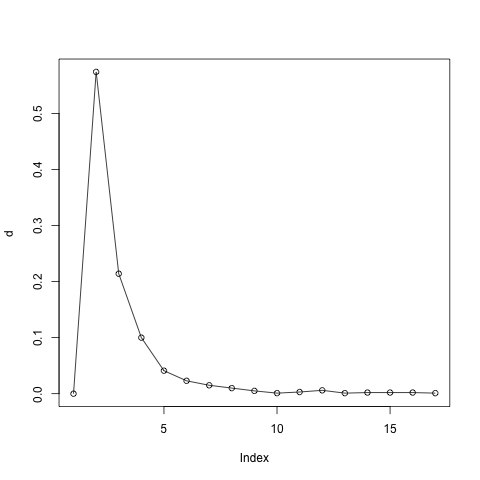
\includegraphics[width=.6\textwidth]{figure2a.png}
\caption{The distribution for fat tailed graph}
\label{fig:sp_hist}
\end{figure}

\subsection{b}
The modularity of the graph is 
We repeated 100 times the graph is always connected.
The GCC is the whole graph.
Number of communities (best split) is 34
The modularity is 0.9348964.

The value of modularity is very big because connections between nodes in different modules are sparse, but between nodes in same modules are dense. 
\subsection{c}
When we build a graph with 10000 nodes, the best split number of community is 105 and the corresponding modularity becomes 0.9792582.
It is greater than the modularity of the case with 1000 nodes.
\subsection{d}
We use histogram to describe the degree distribution.\\
\begin{figure}[htbp]
\centering
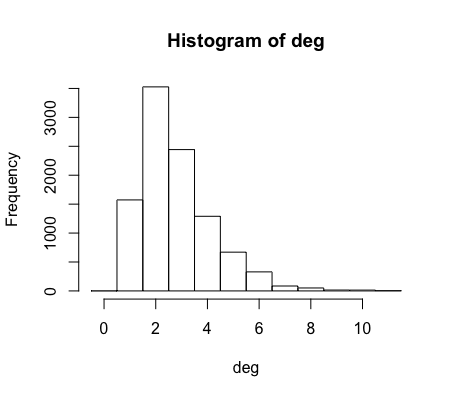
\includegraphics[width=.6\textwidth]{figure2d.png}
\caption{The distribution histogram of degreel}
\label{fig:sp_hist}
\end{figure}
\\
From the graph we can see that, the most common degree is 2.
\end{document}